\documentclass[../Main.tex]{subfiles}

\begin{document}

\IfFileExists{NewCommands.tex}       {% Add new commands here.
%
% Use "providecommand" instead of "newcommand" since we
% want to include this file in all subfiles, and if we
% used newcommand it would report the error
% "Command xxx already defined"
%
%
\providecommand{\dmOT}{\Delta m^2_{\rm 12}}
\providecommand{\dmsolar}{\Delta m^2_{\rm solar}}
\providecommand{\dmatm}{\Delta m^2_{\rm atm}}
\providecommand{\dmTT}{\Delta m^2_{\rm atm}}
\providecommand{\dmsq}[1]{\Delta m^{2}_{#1}}
\providecommand{\thatm}{\Delta m^2_{\rm atm}}
\providecommand{\thTT}{\theta_{\rm 23}}
\providecommand{\sinsq}[1]{\sin^{2}(\theta_{#1})}
\providecommand{\sinsqOT}{\sin^{2}(\theta_{\rm 12})}
\providecommand{\sinsqsolar}{\sin^{2}(\theta_{\rm solar})}
\providecommand{\sinsqTT}{\sin^{2}(\theta_{\rm 23})}
\providecommand{\sinsqTwoTT}{\sin^{2}(2\theta_{\rm 23})}
\providecommand{\dcp}{\delta_{\rm CP}}

\providecommand{\gsim}{\gtrsim}
\providecommand{\lsim}{\lesssim}
\providecommand{\Enu}{\rm{E}_\nu}
\providecommand{\Emu}{\rm{E}_\mu}
\providecommand{\Ecasc}{\rm{E}_{\rm casc}}
\providecommand{\Lmu}{\rm{L}_\mu}
\providecommand{\Lnu}{\rm{L}_\nu}
\providecommand{\Thetamu}{\theta_\mu}
\providecommand{\cosThetamu}{\cos{\theta_\mu}}
\providecommand{\cosThetanu}{\cos{\theta_\nu}}
\providecommand{\Thetanu}{\theta_\nu}
\providecommand{\nue}{\nu_{\rm e}}
\providecommand{\numu}{\nu_\mu}
\providecommand{\nutau}{\nu_\tau}

\providecommand{\ket}[1]{|#1\rangle}

\providecommand{\ue}[1]{|U_{e #1}|}
\providecommand{\umu}[1]{|U_{\mu #1}|}
\providecommand{\utau}[1]{|U_{\tau #1}|}
\providecommand{\uesq}[1]{|U_{e #1}|^{2}}
\providecommand{\umusq}[1]{|U_{\mu #1}|^{2}}
\providecommand{\utausq}[1]{|U_{\tau #1}|^{2}}

\providecommand{\Nch}{${\rm N}_{\rm ch}\,$}
\providecommand{\Ndir}{${\rm N}_{\rm dir}\,$}
\providecommand{\Nstr}{${\rm N}_{\rm str}\,$}
\providecommand{\Aeff}{${\rm A}_{\rm eff}\,$}
\providecommand{\Veff}{${\rm V}_{\rm eff}\,$}
\providecommand{\VeffNS}{${\rm V}_{\rm eff}$}

\providecommand{\pe}{$p.e.$ }
}       {}
\IfFileExists{../NewCommands.tex}    {% Add new commands here.
%
% Use "providecommand" instead of "newcommand" since we
% want to include this file in all subfiles, and if we
% used newcommand it would report the error
% "Command xxx already defined"
%
%
\providecommand{\dmOT}{\Delta m^2_{\rm 12}}
\providecommand{\dmsolar}{\Delta m^2_{\rm solar}}
\providecommand{\dmatm}{\Delta m^2_{\rm atm}}
\providecommand{\dmTT}{\Delta m^2_{\rm atm}}
\providecommand{\dmsq}[1]{\Delta m^{2}_{#1}}
\providecommand{\thatm}{\Delta m^2_{\rm atm}}
\providecommand{\thTT}{\theta_{\rm 23}}
\providecommand{\sinsq}[1]{\sin^{2}(\theta_{#1})}
\providecommand{\sinsqOT}{\sin^{2}(\theta_{\rm 12})}
\providecommand{\sinsqsolar}{\sin^{2}(\theta_{\rm solar})}
\providecommand{\sinsqTT}{\sin^{2}(\theta_{\rm 23})}
\providecommand{\sinsqTwoTT}{\sin^{2}(2\theta_{\rm 23})}
\providecommand{\dcp}{\delta_{\rm CP}}

\providecommand{\gsim}{\gtrsim}
\providecommand{\lsim}{\lesssim}
\providecommand{\Enu}{\rm{E}_\nu}
\providecommand{\Emu}{\rm{E}_\mu}
\providecommand{\Ecasc}{\rm{E}_{\rm casc}}
\providecommand{\Lmu}{\rm{L}_\mu}
\providecommand{\Lnu}{\rm{L}_\nu}
\providecommand{\Thetamu}{\theta_\mu}
\providecommand{\cosThetamu}{\cos{\theta_\mu}}
\providecommand{\cosThetanu}{\cos{\theta_\nu}}
\providecommand{\Thetanu}{\theta_\nu}
\providecommand{\nue}{\nu_{\rm e}}
\providecommand{\numu}{\nu_\mu}
\providecommand{\nutau}{\nu_\tau}

\providecommand{\ket}[1]{|#1\rangle}

\providecommand{\ue}[1]{|U_{e #1}|}
\providecommand{\umu}[1]{|U_{\mu #1}|}
\providecommand{\utau}[1]{|U_{\tau #1}|}
\providecommand{\uesq}[1]{|U_{e #1}|^{2}}
\providecommand{\umusq}[1]{|U_{\mu #1}|^{2}}
\providecommand{\utausq}[1]{|U_{\tau #1}|^{2}}

\providecommand{\Nch}{${\rm N}_{\rm ch}\,$}
\providecommand{\Ndir}{${\rm N}_{\rm dir}\,$}
\providecommand{\Nstr}{${\rm N}_{\rm str}\,$}
\providecommand{\Aeff}{${\rm A}_{\rm eff}\,$}
\providecommand{\Veff}{${\rm V}_{\rm eff}\,$}
\providecommand{\VeffNS}{${\rm V}_{\rm eff}$}

\providecommand{\pe}{$p.e.$ }
}    {}
\IfFileExists{../../NewCommands.tex} {% Add new commands here.
%
% Use "providecommand" instead of "newcommand" since we
% want to include this file in all subfiles, and if we
% used newcommand it would report the error
% "Command xxx already defined"
%
%
\providecommand{\dmOT}{\Delta m^2_{\rm 12}}
\providecommand{\dmsolar}{\Delta m^2_{\rm solar}}
\providecommand{\dmatm}{\Delta m^2_{\rm atm}}
\providecommand{\dmTT}{\Delta m^2_{\rm atm}}
\providecommand{\dmsq}[1]{\Delta m^{2}_{#1}}
\providecommand{\thatm}{\Delta m^2_{\rm atm}}
\providecommand{\thTT}{\theta_{\rm 23}}
\providecommand{\sinsq}[1]{\sin^{2}(\theta_{#1})}
\providecommand{\sinsqOT}{\sin^{2}(\theta_{\rm 12})}
\providecommand{\sinsqsolar}{\sin^{2}(\theta_{\rm solar})}
\providecommand{\sinsqTT}{\sin^{2}(\theta_{\rm 23})}
\providecommand{\sinsqTwoTT}{\sin^{2}(2\theta_{\rm 23})}
\providecommand{\dcp}{\delta_{\rm CP}}

\providecommand{\gsim}{\gtrsim}
\providecommand{\lsim}{\lesssim}
\providecommand{\Enu}{\rm{E}_\nu}
\providecommand{\Emu}{\rm{E}_\mu}
\providecommand{\Ecasc}{\rm{E}_{\rm casc}}
\providecommand{\Lmu}{\rm{L}_\mu}
\providecommand{\Lnu}{\rm{L}_\nu}
\providecommand{\Thetamu}{\theta_\mu}
\providecommand{\cosThetamu}{\cos{\theta_\mu}}
\providecommand{\cosThetanu}{\cos{\theta_\nu}}
\providecommand{\Thetanu}{\theta_\nu}
\providecommand{\nue}{\nu_{\rm e}}
\providecommand{\numu}{\nu_\mu}
\providecommand{\nutau}{\nu_\tau}

\providecommand{\ket}[1]{|#1\rangle}

\providecommand{\ue}[1]{|U_{e #1}|}
\providecommand{\umu}[1]{|U_{\mu #1}|}
\providecommand{\utau}[1]{|U_{\tau #1}|}
\providecommand{\uesq}[1]{|U_{e #1}|^{2}}
\providecommand{\umusq}[1]{|U_{\mu #1}|^{2}}
\providecommand{\utausq}[1]{|U_{\tau #1}|^{2}}

\providecommand{\Nch}{${\rm N}_{\rm ch}\,$}
\providecommand{\Ndir}{${\rm N}_{\rm dir}\,$}
\providecommand{\Nstr}{${\rm N}_{\rm str}\,$}
\providecommand{\Aeff}{${\rm A}_{\rm eff}\,$}
\providecommand{\Veff}{${\rm V}_{\rm eff}\,$}
\providecommand{\VeffNS}{${\rm V}_{\rm eff}$}

\providecommand{\pe}{$p.e.$ }
} {}


\graphicspath{{figures/}{Reconstructions/figures/}}


\section{Reconstructions}\label{sec:Reconstructions}

Here we are going to write some really good words about the
reconstructions, at least the higher level reconstructions.

Performance of the reconstructions is given at the end

\subsection{Single String ANTares inspired Algorithm}\label{sec:SANTA}
This directional fit follows the one introduced first by J. Brunner \textit{et al.} in \cite{bbfit} (ANTARES). We use the same terminology and notation as in the original paper, with minor modifications. The diagram of Fig.\,\ref{fig:santa_sketch} shows the variables described below.

\subsubsection{Track-like sources}
Starting from the assumption that a particle travels at a known constant speed and it does so in a straight path, there are six variables that completely define its kinematical behavior: a point in space time along the particle's trajectory, and two angles which determine its direction. While the two angles are unique, the point along the trajectory of the particle contains a redundant variable, as any point can be chosen. All these points that form part of the track's trajectory can be parameterized as
\begin{equation}
\vec{p}(t) = \vec{q} + c\left( t-t_0 \right) \vec{u}\,,
\end{equation}
where $\vec{q}$ is the point crossed at $t_0$ and $\vec{u}$ is the direction vector, given by
\begin{equation}
  \vec{u} = \{ \cos\vartheta \cos\phi, \, \cos\vartheta\sin\phi,\, \sin\vartheta \}\,.
  \label{eq:udef}
\end{equation}
Note that in Eq.\,\ref{eq:udef} the zenith angle appears in $\vartheta = \theta_z - \pi/2$.

Approximating the strings as vertical lines parallel the $z$-axis at positions $(L_x,\,L_y)$, the coordinates of the point of closest approach are given by this set of formulas,
\begin{align}
z_c &= \frac{q_z - u_z \left( \vec{q}\cdot\vec{u}\right) + u_z \left( L_x u_x + L_y u_y\right)}{1-u^2_z}\,,\\
t_c &= t_0 + \frac{1}{c} \left( L_x u_x + L_y u_y + q_z u_z - \vec{q}\cdot\vec{u} \right)\,, \\
d_c &= \sqrt{\left( p_{x}(t_c) - L_x  \right)^2 + \left( p_{y}(t_c) - L_y \right)^2}\,.
\label{eq:hyperbola_third_eq}
\end{align}
Here the track has been conveniently parameterized in terms of the quantities which define the hyperbola of Fig.\,\ref{fig:santa_sketch}: $z_c$, $t_c$, $d_c$ and $u_z$.

In the case of dealing with a single string there is no preferred direction in the $x-y$ plane, and the symmetry makes the quantities defined useful, as they fully define the particle track. Dealing with one string only allows for the freedom to redefine the $x$ and $y$ coordinates of its position. Setting the $x-y$ position of the string to $(0,0)$ ($L_x = 0, L_y = 0)$ simplifies the equations, giving
\begin{align}
z_c &= \frac{q_z - u_z \left( \vec{q}\cdot\vec{u}\right)}{1-u^2_z}\,,\\
t_c &= t_0 + \frac{1}{c} \left( q_z u_z - \vec{q}\cdot\vec{u} \right)\,, \\
d_c &= \sqrt{ p^2_x + p^2_y }\,.
\end{align}

% Continue with ANTARES' paper
Using these variables, the time of arrival of a photon $t_\gamma$ at a point $z$ along the string, which experiences a refraction index $n$, can be calculated by
\begin{align}
t_\gamma(z) = \left(t_c - t_0 \right) + \frac{1}{c} \left( \left(z-z_c\right) u_z + \frac{n^2 -1}{n} d_\gamma(z) \right)\,, \\
d_\gamma(z) = \frac{n}{\sqrt{n^2-1}} \sqrt{d^2_c + (z-z_c)^2\,(1-u_z^2)}\,,\\
\cos \theta_\gamma(z) = \left( 1-u_z^2\right)^2 \frac{z-z_c}{d_\gamma(z)} + \frac{u_z}{n}\,.
\end{align}
The variables $d_\gamma$ and $\theta_\gamma$ are the distance traveled by the photon and the angle of arrival with respect to the string's axis, as shown in Fig.\,\ref{fig:santa_sketch}. The equations are valid if there are pulses in multiple strings as well. This requires (i) that the differences in string positions are taken into account, and (ii) an extra variable to fully define the problem, as there is no rotational symmetry any longer.

\subsubsection{Point-like sources}
The emission of an isotropic point-like source, which produces a single light flash at a given moment, is also described by a hyperbola. This approximation can be used to model cascades because their elongation is much shorter than the spacing between DOMs, even in the DeepCore volume.

Unlike for the track case, a point-like isotropic emitter does not have a travel direction, thus the problem has one degree of freedom less. It is convenient to modify the point of closest approach to represent the interaction vertex of a cascade, then $z_c = q_z$, $t_c = t_0$, and 
\begin{equation}
d_c = \sqrt{(q_x - L_x)^2 + (q_y - L_y)^2}\,.
\end{equation}
Considering a single string again, and assuming that it is located at $(0,0)$, then $d_c = \sqrt{q_x^2 + q_y^2}$. The photon arrival time $t_\gamma$ is now given by a different set of equations:
\begin{align}
t_\gamma(z) = t_0 + \frac{n}{c} d_\gamma\,,\\
d_\gamma(z) = \sqrt{d_c^2 + (z-q_z)^2}\,,\\
\cos \varphi_\gamma (z) = \frac{z-q_z}{d_\gamma}\,.
\end{align}
Again, multiple strings can be used, as long as the simplification of putting them at (0,0) is removed.

\subsubsection{Fitting procedure}
In order to fit the observed time of arrival with the expectation we use a $\chi^2$ with an additional term. The error involved in the observation is estimated by the readout binsize of 3\,ns. The errors are expected to follow a normal distribution, which justifies the method selected.

The timing information is complemented by using the total charge observed at each DOM. For a medium with uniform optical properties the largest signal is expected from the photons that travel the shortest distances to the detection unit. This is implemented by including a term that penalizes trajectories in which this does not hold. For this purpose the angular acceptance of the DOM needs to be included, which is modeled as $(\cos \theta_\gamma + 1)/2$, where $\theta_\gamma$ is the polar angle defined by the axis of the DOM. The measured charge $q_i$ in the $i$-th DOM is corrected as
\begin{equation}
q'_i = \frac{2q_i}{\cos \varphi_\gamma + 1}\,.
\end{equation}

There is a minimum distance which any photon travels $d_\mathrm{min}$, given by the DOM size itself. Enforcing it avoids the tendency to systematically put the track fit close to a detector string. This is done by using a modified photon travel distance $D$, which is defined as
\begin{equation}
 D(d_\gamma) \equiv \sqrt{d_\mathrm{min}^2 + d_\gamma^2}\,.
\end{equation}

The modified $\chi^2$ is then
\begin{equation}
\chi^2_\mathrm{mod} = \sum_{i=1} \left[ \frac{(t_{\gamma, \mathrm{exp}}(z_i) - t_{\gamma,\mathrm{obs}} (z_i))^2}{\sigma_\gamma^2} + \frac{q'(z_i)\,D(d_\gamma)}{\bar{q}\,d_0}\right]\,.
\label{eq:mod_chi2}
\end{equation}
Here the expected and observed time of arrivals $t_\gamma$ are compared, in units of the time resolution $\sigma_\gamma^2$. The integrated and corrected charge $q'_i$ multiplied by the travel distance $D$ is weighted by the mean charge $\bar{q}$ multiplied by $d_0$. This quantity, $d_0$, enters to balance the weight between the two terms, and can be interpreted as the typical distance at which the detector expects to see a signal of one photoelectron. The values used for this work are $\sigma_\gamma = 3$\,ns, taken from PMT calibration studies \cite{icecube_pmt}, and $d_0 = 10$\,m, taken from simulation.

\subsection{FiniteReco}\label{sec:FiniteReco}
The cascade develops fully in a distance of a few meters. After that, all light that can be detected comes from the muon track. The emission follows the sharp profile shown previously in Fig \ref{fig:LightProfile}. If the muon decays inside the detector, its range can be used to determine the initial energy that it carried (Eq.\,\ref{eq:MuLossSimple}). If the muon leaves the detector, the same Equation can be used too place a lower limit on the muon energy.

The first guess for the position where the muon decays is obtained by projecting the DOMs onto the track direction using the Cherenkov angle. The last point where a projection is found is used. This point is given as a seed to a more sophisticated method that includes the expected pulses from a muon track, as described in \cite{freco}.

The probabilities for observing and not observing a signal given that there was a track present are calculated and combined in the likelihood ratio
\begin{equation}
\mathrm{LLHR} = \ln\frac{P(\mathrm{noHit} | \mathrm{Track})}{P(\mathrm{noHit}| \mathrm{noTrack})}\,.
\label{eq:fReco_LLH}
\end{equation}
Here $P(\mathrm{noHit} | \mathrm{Track})$ is the probability for not observing the light from the track, and $P(\mathrm{noHit} | \mathrm{noTrack})$ is the probability of not detecting photons given that the track decayed at an earlier point. Both situations are exemplified in Fig.\,\ref{fig:fReco_LLH}. The ratio in Eq.\,\ref{eq:fReco_LLH} is minimized to identify the most likely decay point of the muon track being considered. 

\begin{figure}[tbh]
  \centering
  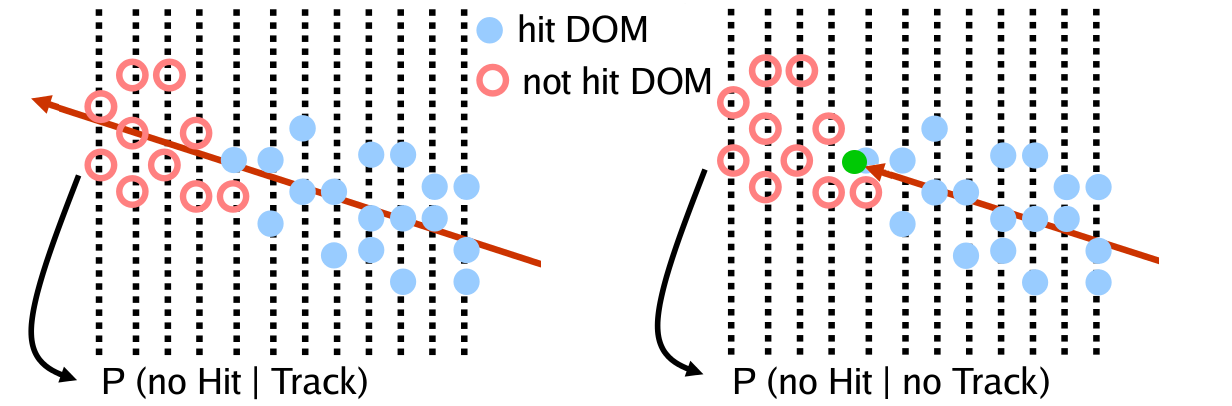
\includegraphics[width=0.9\textwidth]{finiteReco3}
  \caption[Determining the muon decay point.]{Sketch of how the probabilities to determine the position where the muon decays are calculated. The point of muon decay is marked in green (right-hand figure).}
  \label{fig:fReco_LLH}
\end{figure}

\vspace*{\baselineskip}
The range of the muon is calculated from the separation between the interaction vertex and the most likely decay point. By means of Eq.\,\ref{eq:MuLossSimple} the range can be converted into the initial muon energy, solving part of the problem. The next step is to estimate the cascade energy, but before doing so, the light contribution from the track has to be disentangled from the contribution of the cascade.

\subsection{LEERA}\label{sec:LEERA}

\textbf{Andrii}

\begin{itemize}
\item Aim of the code
\item Strategy (what to fit and how, assumptions)
\item Fitting function
\item Performance
\end{itemize}

\subsection{HybridReco/PegLeg}\label{sec:HybridReco}

\begin{itemize}
\item Aim of the code
\item Strategy (what to fit and how, assumptions)
\item Fitting function
\item PegLeg implementation
\item Minimization procedure (MultiNest)
\item Performance
\end{itemize}

\subsubsection{MultiNest}\label{sec:MultiNest}

\subsubsection{PegLeg}\label{sec:PegLeg}

\subsubsection{Monopod?}\label{sec:Monopod}

\textbf{Has anybody used this?}

\subsection{Reconstruction performance}\label{sec:reco_performance}

Discuss and tabulate, show figures for
\begin{itemize}
\item The percentage of events that a reconstruction can handle as function of Nhit (clean)
\item The average time an event takes to reconstruct
\item The error on the zenith angle for the directional recos. Show plots a-la-Dunkmann and the tails using a CDF
\item The relative error on the energy, using same strategy
\item Show this for tracks and cascade-like events?
\end{itemize}


%\begin{figure}
%\centering
%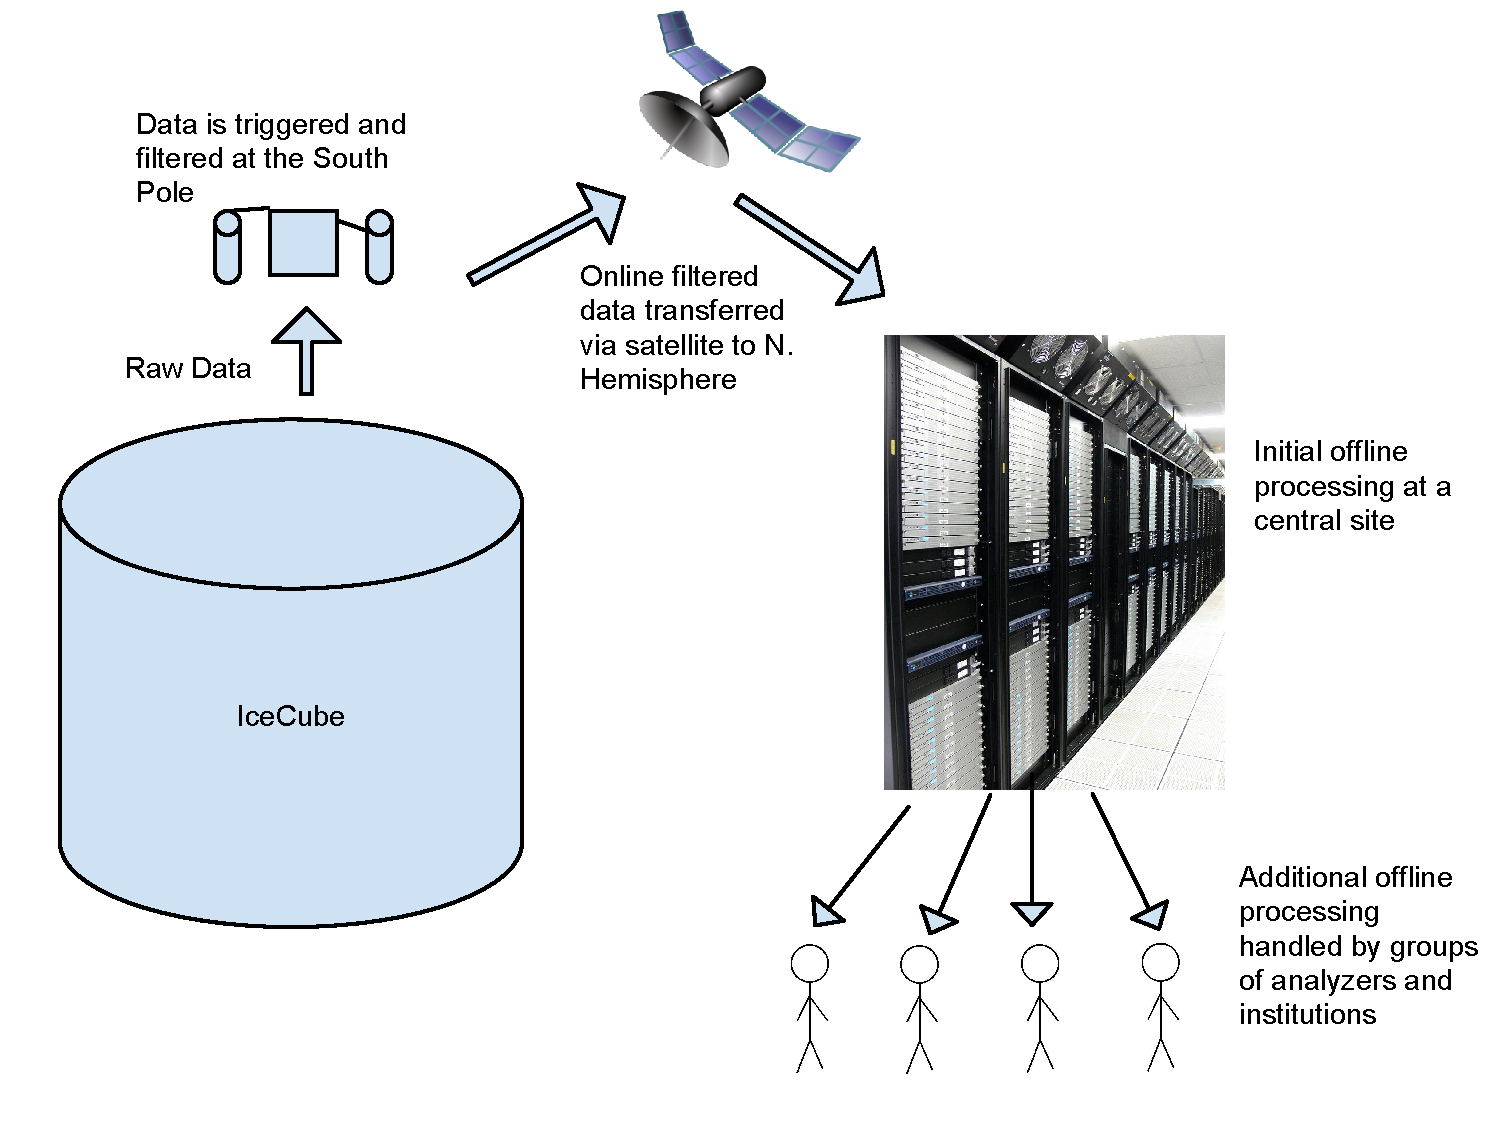
\includegraphics[scale=0.4]{Online_IceCube_data_processing_flow_chart.pdf}
%\caption{\label{fig:DataFlowChart} Should we include, an obviously
%  nicer, flow chart of data collection? More simple? Redundant because
%it'll be in the IceCube Detector paper?}
%\end{figure}

\end{document}
